\chapter{Vymedzenie problému a návrh riešenia}
\label{chapter:problem}

\section{Vymedzenie problému}
\label{sec:problem}

Slovenské školy stoja pred rozhodnutím, ktoré musia urobiť bez dôkazov. Od marca 2026 je gramotnosť v oblasti umelej inteligencie súčasťou Štátneho vzdelávacieho programu pre základné školy a v školskom roku 2026/2027 sa má rozšíriť na stredné školy~\cite{minedu2025plan}; súčasne je plánované sprístupnenie desiatok tisíc licencií na konverzačné systémy pre pedagógov~\cite{drucker2026competence}. Otázka teda už neznie, \emph{či} sa nástroje umelej inteligencie do vyučovania dostanú, ale \emph{v akej podobe}.

Na túto otázku súčasná literatúra neposkytuje jednoznačnú odpoveď a v slovenskom kontexte neposkytuje žiadnu~--- systematická rešerš 155 empirických štúdií~\cite{garzon2025systematic} nenašla zo Slovenska ani jednu prácu spĺňajúcu kritériá zaradenia. Zahraničné zistenia si navyše zdanlivo protirečia: adaptívny tutor prekonáva aktívne učenie~\cite{kestin2025aitutoring}, generatívny nástroj však znižuje výsledky na následnom teste~\cite{bastani2025harm}.

Problém, ktorý táto práca rieši, má dve vrstvy. \textbf{Vecná vrstva:} nie je známe, či a za akých podmienok nástroj umelej inteligencie podporuje \emph{trvalé} osvojenie učiva u slovenských stredoškolákov, a či sa v tom líši generický nástroj od pedagogicky ohraničeného. \textbf{Metodologická vrstva:} chýba merací nástroj, ktorým by bolo možné charakter interakcie žiaka s modelom zistiť \emph{pozorovaním} namiesto sebahodnotenia~--- a práve táto veličina je podľa syntézy v časti~\ref{sec:syntezahypotezy} kľúčom k vysvetleniu rozporov v literatúre.

Bez vyriešenia druhej vrstvy nemožno spoľahlivo odpovedať na prvú. Sebahodnotiace škály zlyhávajú práve pri správaní, ktoré žiak nemá dôvod priznať a ktorého si nemusí byť vedomý; EEG je v triede nepoužiteľné. Práca preto rieši obidve vrstvy súčasne: navrhuje merací nástroj a používa ho v experimente, ktorý bez neho nie je uskutočniteľný.

\section{Prehľad technickej literatúry}
\label{sec:techlit}

Technická úloha znie: zachytiť obsah dopytov, ktoré žiak odosiela konverzačnému systému cez prehliadač, na školskom zariadení, transparentne a v súlade s ochranou osobných údajov. Existujúce riešenia možno rozdeliť do štyroch tried.

\paragraph{Rozšírenia prehliadača.} Najjednoduchšia cesta: obsahový skript číta text z rozhrania. Silná stránka je jednoduchosť a to, že rozšírenie vidí presne to, čo vidí žiak. Slabinou je krehkosť~--- akákoľvek zmena rozhrania poskytovateľa rozšírenie rozbije~--- a viazanosť na jeden prehliadač a jednu službu. Pre longitudinálny zber cez viacero služieb je to neudržateľné.

\paragraph{Prístup cez rozhranie poskytovateľa (API).} Metodologicky najčistejšie, pretože dáta sú štruktúrované. Nevýhodou je zásadná strata ekologickej validity: žiak by nepoužíval nástroj, ktorý používa doma, ale výskumnú aplikáciu. Meral by sa iný jav. Tento prístup je pritom v podmienke $A$ nevyhnutný~--- adaptívnu vrstvu inak nemožno vložiť~--- ale pre podmienku $G$ by zmaril samotný účel.

\paragraph{Sieťová telemetria.} Analýza metadát toku (adresy, objemy, časovanie) bez dešifrovania. Neinvazívne, ale poskytuje len to, \emph{že} žiak komunikoval, nie \emph{čo} poslal. Pre výpočet PEQI je to nepoužiteľné.

\paragraph{Lokálny sprostredkujúci server s termináciou TLS.} Zvolené riešenie. Prehliadač komunikuje cez lokálny proxy server, ktorý ukončí TLS pomocou vlastnej certifikačnej autority nainštalovanej na zariadení, prečíta telo požiadavky, porovná cieľovú adresu so zoznamom povolených a zhodné požiadavky zapíše. Táto trieda riešení je dobre preskúmaná v oblasti bezpečnostného testovania a poskytuje nezávislosť od prehliadača aj od zmien rozhrania. Cenou je zásah, ktorý musí byť transparentný a časovo aj priestorovo ohraničený, čomu sa venuje príloha~\ref{chapter:etika}.

Porovnanie štyroch tried podľa kritérií, ktoré sú pre túto prácu rozhodujúce, je v tabuľke~\ref{tab:zber-porovnanie}.

\begin{table}[H]
\centering
\caption{Porovnanie prístupov k zberu údajov o interakcii žiaka s konverzačným systémom}
\label{tab:zber-porovnanie}
\footnotesize
\begin{tabularx}{\textwidth}{@{}p{2.6cm} c c c c X@{}}
\toprule
\textbf{Prístup} & \textbf{Obsah} & \textbf{Ekolog. validita} & \textbf{Odolnosť} & \textbf{Zásah} & \textbf{Záver} \\
\midrule
Rozšírenie prehliadača & áno & vysoká & nízka & malý & krehké pri zmenách rozhrania \\
Rozhranie poskytovateľa & áno & nízka & vysoká & žiadny & vhodné len pre podmienku $A$ \\
Sieťová telemetria & nie & vysoká & vysoká & malý & nestačí na výpočet PEQI \\
\textbf{Lokálny proxy s TLS} & \textbf{áno} & \textbf{vysoká} & \textbf{stredná} & \textbf{veľký} & \textbf{zvolené; vyžaduje etické ošetrenie} \\
\bottomrule
\end{tabularx}
\end{table}

V rámci zvolenej triedy bolo potrebné vybrať konkrétnu knižnicu. Prvá implementácia použila LittleProxy s rozšírením littleproxy-mitm v jazyku Java. Toto rozhodnutie sa ukázalo ako chybné a dôvody sú predmetom nasledujúcej časti; alternatívou, ktorá obstála, je mitmproxy~\cite{mitmproxy}.

\section{Návrh riešenia}
\label{sec:riesenie}

\subsection{Prvá iterácia a jej overenie}

V prvom semestri bola implementovaná overovacia kostra (\emph{walking skeleton}): nástroj príkazového riadka v jazyku Java, ktorý spustí lokálny proxy server na adrese \texttt{127.0.0.1}\discretionary{}{}{}\texttt{:8080}, terminuje TLS vlastnou certifikačnou autoritou importovanou do prehliadača Firefox, porovnáva cieľové adresy so zoznamom povolených načítaným z konfiguračného súboru YAML a telá zhodných požiadaviek zapisuje do súborov vo formáte JSON Lines. Súčasťou je aj samostatný príkaz na generovanie súhrnnej správy zo zachytených údajov.

Kostra bola overená voči službe ChatGPT. Výsledok overenia bol \emph{čiastočne negatívny} a práve preto je cenný. Zachytené boli požiadavky typu automatického dopĺňania a prípravy konverzácie. Koncový bod odosielajúci samotnú správu však vrátil chybu 400 priamo na úrovni proxy servera a odpovede prenášané cez WebSocket neboli zachytené vôbec.

Analýza príčiny ukázala, že nejde o chybu v aplikačnej logike, ale o obmedzenie zvolenej knižnice: LittleProxy vo verzii používanej od roku 2019 nepodporuje HTTP/2 ani tunelovanie WebSocket cez terminovaný TLS. Moderné konverzačné rozhrania obidve technológie používajú. Chyba bola teda v rozhodnutí o výbere knižnice, nie v jej použití.

\paragraph{Metodologická poznámka.} Hodnota overovacej kostry spočíva presne v tomto: odhalila nevhodnosť základnej technologickej voľby v okamihu, keď ju bolo možné zmeniť za cenu jedného semestra, a nie po nasadení do škôl, keď by to znamenalo stratu celého zberu dát. Negatívny výsledok overenia je preto vykazovaný ako plnohodnotný výsledok prvej fázy.

\subsection{Druhá iterácia: rozdelenie zodpovedností}

Revidovaná architektúra vymieňa záchytnú vrstvu, ale zachováva aplikačnú. Výmena je motivovaná tým, že mitmproxy~\cite{mitmproxy} je aktívne udržiavaný, podporuje HTTP/2, HTTP/3 aj WebSocket a má stabilné rozhranie pre doplnky. Zachovanie aplikačnej vrstvy v Jave je motivované tým, že práve tam je uložená logika, ktorá je predmetom práce~--- pseudonymizácia, odstraňovanie osobných údajov, výpočet PEQI~--- a tá s voľbou proxy servera nesúvisí.

\begin{figure}[H]
    \centering
    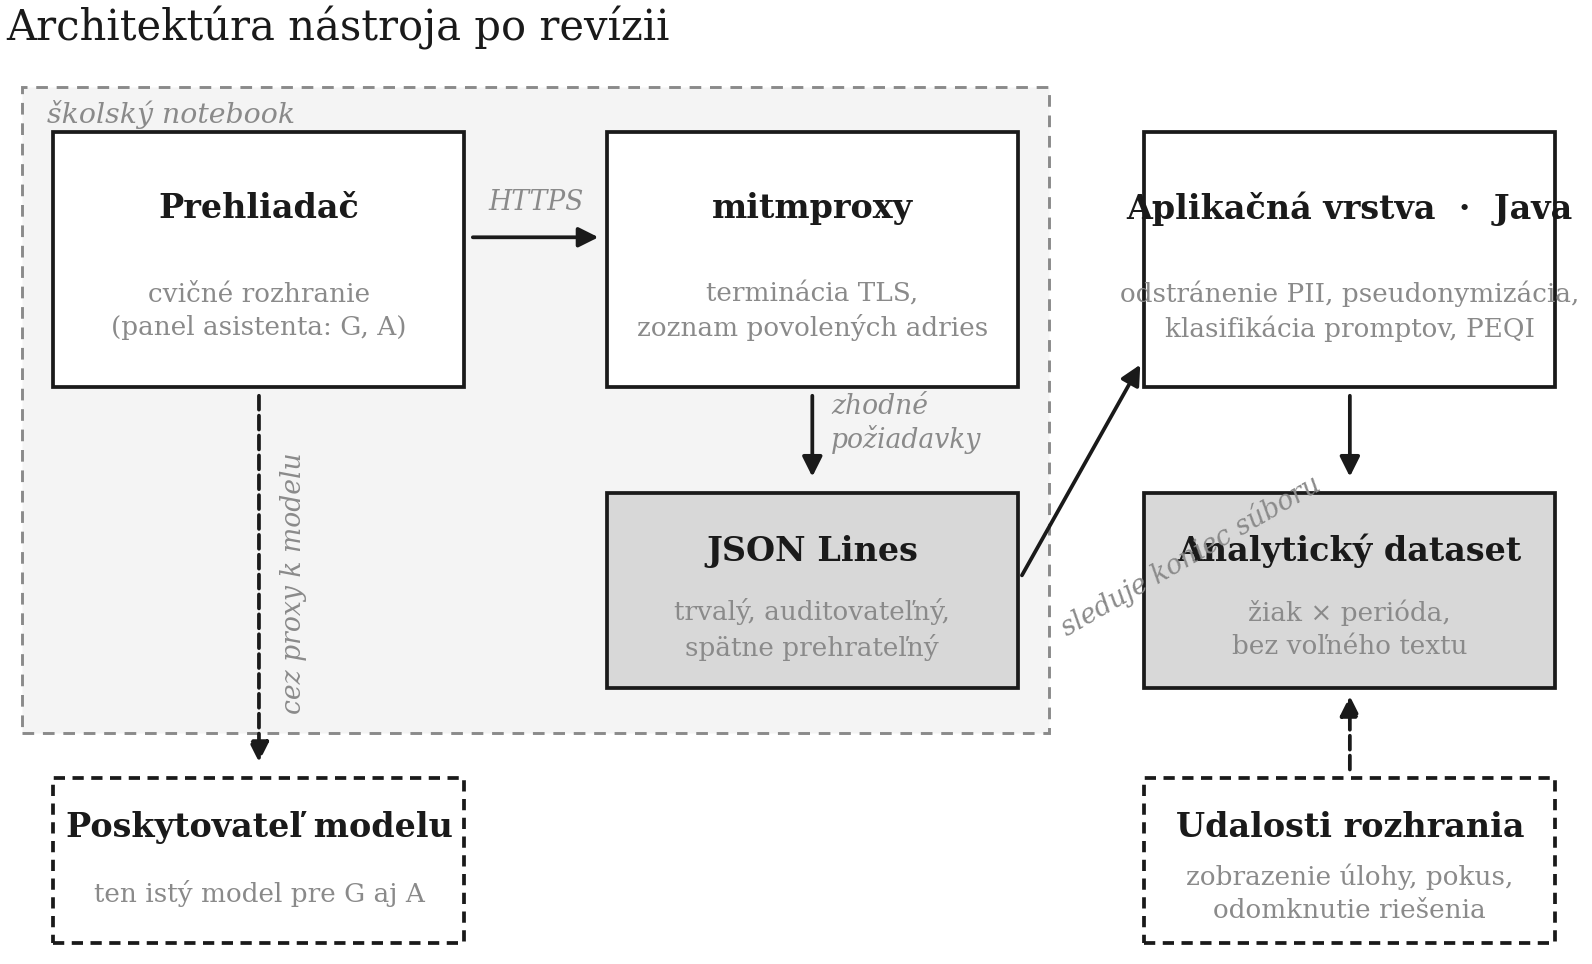
\includegraphics[width=\textwidth]{assets/images/fig_architecture.png}
    \caption{Architektúra nástroja po revízii. Záchytná vrstva je vymenená za mitmproxy; aplikačná vrstva v Jave zostáva a komunikuje s ňou cez súbor JSON Lines, ktorý slúži zároveň ako trvalý záznam pre audit.}
    \label{fig:architektura}
\end{figure}

Vrstvy a ich zodpovednosti:

\begin{description}[leftmargin=2.6cm, style=nextline, nosep]
    \item[Záchytná vrstva] Doplnok k mitmproxy v jazyku Python. Filtruje požiadavky podľa zoznamu povolených adries, extrahuje telo, pripája časovú značku a pseudonym relácie a zapisuje jeden riadok JSON na požiadavku. Nerobí nič iné~--- zámerne, aby bola vymeniteľná.
    \item[Prepojenie] Súbor JSON Lines s pripájaním na koniec. Voľba súboru namiesto priameho volania alebo soketu je zámerná: prežije pád ktorejkoľvek strany, je čitateľný bez nástrojov, umožňuje spätné prehratie celého zberu pri zmene výpočtu ukazovateľov a je priamo auditovateľný~--- škola si môže pozrieť, čo presne sa zachytilo.
    \item[Aplikačná vrstva] Java. Číta súbor, klasifikuje prompty podľa taxonómie z prílohy~\ref{chapter:kodovaci-manual}, počíta PEQI a odvodené ukazovatele a zapisuje analytický dataset na úrovni žiak~$\times$~relácia. Je implementovaná ako podpríkaz \texttt{peqi} a pokrytá 41~jednotkovými testami, v ktorých sú kotviace príklady z kódovacieho manuálu zapísané ako testovacie prípady~--- manuál a kód tak nemôžu nepozorovane rozísť. Odstraňovanie osobných údajov a pseudonymizácia prebiehajú už v záchytnej vrstve, teda \emph{pred} zápisom na disk, aby sa neošetrený text nikdy neuložil.
    \item[Cvičné rozhranie] Webová aplikácia so zadaniami, ktorá obsluhuje všetky tri podmienky (časť~\ref{sec:cvicne-rozhranie}). Dodáva udalosti neviditeľné v sieťovej prevádzke: zobrazenie úlohy, prvé stlačenie klávesu, odoslanie pokusu, odomknutie riešenia. Zapisuje ich v tom istom formáte JSON Lines ako záchytná vrstva, takže aplikačná vrstva číta oba zdroje bez toho, aby vedela, ktorý ich vytvoril. Bez nich nie je možné vypočítať $T_1$ ani ABHR: sieť nevidí, že žiak čítal zadanie deväťdesiat sekúnd, ani že to už dvakrát skúsil.
\end{description}

\subsection{Cvičné rozhranie a pedagogická vrstva podmienky A}
\label{sec:cvicne-rozhranie}

Všetky tri podmienky obsluhuje \emph{jeden} program. Nejde o pohodlie, ale o kontrolu: ak by kontrolná podmienka bežala na inom softvéri, akýkoľvek rozdiel medzi podmienkami by zamieňal pedagogiku so všetkým ostatným, čo softvér robí, a hlavné tvrdenie dizajnu by nebolo overiteľné.

Podmienky $G$ a $A$ sa líšia presne na dvoch miestach v obsluhe jedného koncového bodu: aký zoznam správ sa zostaví a či odpoveď prechádza výstupnou kontrolou. Všetko ostatné~--- úlohy, rozloženie, časovanie, záznam udalostí~--- je zdieľané a identické. Toto tvrdenie nie je vyslovené, ale \emph{testované}: test porovnáva, čo každá podmienka skutočne odosiela modelu, a overuje, že sa líšia len prítomnosťou systémového promptu.

\paragraph{Tri mechanizmy podmienky A.} Systémový prompt zakazujúci hotové riešenie a vynucujúci stupňované nápovede (príloha~\ref{sec:sysprompt}); štvorparametrový model sledovania znalostí (Bayesian knowledge tracing) pre každú z piatich čiastkových zručností, ktorý riadi výber ďalšej úlohy aj stupeň, na ktorom nápoveda začína; a brána vlastného vysvetlenia pred odomknutím vzorového riešenia.

\paragraph{Výstupná kontrola, a prečo nestačí systémový prompt.} Systémový prompt je požiadavka, nie obmedzenie. Model ho väčšinou dodrží, a „väčšinou“ nestačí, keď od neho závisí rozdiel medzi dvoma experimentálnymi podmienkami. Každá odpoveď v podmienke $A$ preto prechádza aj strojovou kontrolou na prítomnosť blokov kódu, úplných definícií funkcií, fráz oznamujúcich výsledok a samotnej referenčnej odpovede. Porušenie sa nahradí otázkou \emph{a zaznamená}, pretože miera, s akou prompt zlyháva, je číslo, ktoré práca musí vykázať, nie podrobnosť, ktorú možno zamlčať.

Podmienkou nasadenia je nulový počet únikov pri sade 40 útočných dopytov (príloha~\ref{sec:sysprompt}). Táto sada je súčasťou testov a v aktuálnej verzii prechádza.

\paragraph{Adaptácia až po dôkaze.} Jedno pravidlo stojí za uvedenie, pretože bolo najprv implementované nesprávne. Prior modelu sledovania znalostí ($0{,}25$) leží zo svojej podstaty \emph{pod} prahom pre vloženie medzikroku ($0{,}40$). Bez ďalšej podmienky by teda každý žiak bol označený za zaostávajúceho skôr, než čokoľvek odpovedal, a dostal by medzikrok hneď pri prvej úlohe~--- čo by adaptivitu úplne zrušilo. Pravidlá sekvencovania sa preto spúšťajú až vtedy, keď pre danú zručnosť existuje aspoň jedno pozorovanie. Adaptovať znamená prispôsobiť sa dôkazu, nie prioru.

\paragraph{Prečo nie hotová platforma.} Khanmigo ani iný komerčný tutor nedovolí manipulovať pedagogickú vrstvu pri konštantnom modeli, obsahu a rozhraní. Bez tejto kontroly by rozdiel medzi podmienkami $G$ a $A$ nebolo možné pripísať pedagogike~--- presne táto zámena je hlavným obmedzením štúdie Slijepcevica a Yaylaliho~\cite{slijepcevic2025khanmigo}.

\subsection{Zdôvodnenie kľúčových technických rozhodnutí}

\begin{table}[H]
\centering
\caption{Kľúčové technické rozhodnutia, ich alternatívy a dôvod voľby}
\label{tab:rozhodnutia}
\small
\begin{tabularx}{\textwidth}{@{}l X X@{}}
\toprule
\textbf{Rozhodnutie} & \textbf{Zvážená alternatíva} & \textbf{Dôvod voľby} \\
\midrule
mitmproxy namiesto LittleProxy & zostať pri Jave a doimplementovať HTTP/2 & podpora HTTP/2, HTTP/3 a WebSocket; aktívna údržba; vlastná implementácia by bola mimo rozsah práce \\
JSON Lines ako prepojenie & gRPC, Unix soket, zdieľaná databáza & odolnosť voči pádu, auditovateľnosť školou, možnosť spätného prehratia \\
Ponechanie aplikačnej vrstvy v Jave & prepísať všetko do Pythonu & logika práce je v nej; prepis by nepriniesol vedeckú hodnotu \\
Klasifikátor na priehľadných príznakoch & jazykový model ako klasifikátor & overiteľnosť zaradenia školou aj oponentom; nezávislosť od externej služby; nižšia cena \\
Certifikát len na školských zariadeniach & inštalácia aj na súkromné zariadenia & zásah do súkromia mimo školy je neprimeraný účelu \\
Neukladanie odpovedí doslovne & ukladať celú konverzáciu & na výpočet VTR postačuje odtlačok a dĺžka; minimalizácia údajov \\
\bottomrule
\end{tabularx}
\end{table}

\section{Posúdenie rizík}
\label{sec:rizika}

Riziká sú zoradené podľa súčinu pravdepodobnosti a dopadu. Uvedené sú len tie, ktoré môžu ohroziť dokončenie práce alebo platnosť jej záverov.

\begin{table}[H]
\centering
\caption{Register rizík so zmierňujúcimi opatreniami}
\label{tab:rizika}
\scriptsize
\begin{tabularx}{\textwidth}{@{}X c c X@{}}
\toprule
\textbf{Riziko} & \textbf{P} & \textbf{D} & \textbf{Zmiernenie} \\
\midrule
Nepodarí sa získať dostatok tried (pod 12) & S & V & Oslovenie štyroch škôl namiesto troch; postavenie STU ako kompetenčného centra~\cite{drucker2026competence}; záložný plán: dvojpodmienkový dizajn $K$ vs. $G$, ktorý pri 9 triedach ešte má silu $0{,}82$ \\
Zmena rozhrania poskytovateľa počas zberu & V & S & Vymeniteľná záchytná vrstva; zoznam adries v konfigurácii; denná kontrola miery pokrytia počas zberu \\
Žiaci použijú vlastné zariadenie & V & S & Meranie miery pokrytia porovnaním s udalosťami cvičného rozhrania; citlivostná analýza; explicitná dohoda so žiakmi \\
Nedostatočná spoľahlivosť odloženého testu & S & V & Pilotné overenie obtiažnosti položiek; rezervná sada položiek; simulačne overená dĺžka testu \\
Odvolanie súhlasu väčšieho počtu žiakov & N & V & Nadhodnotenie cieľovej vzorky o 15\,\%; zrozumiteľný súhlas; možnosť zúčastniť sa hodiny bez zberu dát \\
Výpadok cvičného rozhrania počas hodiny & S & S & Tlačená záložná verzia pracovného listu; hodina pokračuje, stratia sa len procesné ukazovatele \\
Nedostatočná zhoda kódovateľov (pod $0{,}80$) & N & S & Kotviaci súbor s hraničnými prípadmi; spoločné školenie; zlúčenie susedných úrovní ako záložná stratégia \\
Zmena ceny alebo dostupnosti modelu & S & N & Vrstva abstrakcie nad poskytovateľom; rozpočet na základe pilotu; možnosť lokálneho modelu \\
\bottomrule
\end{tabularx}
\vspace{2pt}
\footnotesize P = pravdepodobnosť, D = dopad; N = nízka, S = stredná, V = vysoká.
\end{table}

Najvážnejším rizikom je nedostatok tried, pretože ovplyvňuje samotnú rozhodnuteľnosť hlavného tvrdenia. Preto je preň pripravený vopred definovaný záložný plán: ak sa do začiatku zberu nepodarí získať aspoň 12~tried, dizajn sa zredukuje na dve podmienky ($K$ a $G$), čím sa uvoľní kapacita na tretiu periódu a zvýši počet pozorovaní na kontrast. Toto rozhodnutie musí padnúť \emph{pred} prvým meraním a musí byť zaznamenané v predregistrácii.

\section{Reprodukovateľnosť a integrácia}
\label{sec:reprodukovatelnost}

Reprodukovateľnosť je v tejto práci riešená na štyroch úrovniach, ktoré zodpovedajú štyrom veciam, ktoré môže chcieť niekto iný zopakovať.

\subsection{Zopakovať analýzu}

Celý analytický reťazec je uložený ako spustiteľný kód v priečinku \texttt{analysis/} (príloha~\ref{chapter:sap}). Pozostáva z \repoModules{} modulov: \texttt{dgp.py} (generujúci model), \texttt{pipeline.py} (štatistický plán), \texttt{identification.py} (odhady mechanizmu a analýza citlivosti), \texttt{measurement.py} (chyba merania mediátora), \texttt{power.py} (sila testu), \texttt{validate\_plan.py} (operačné charakteristiky plánu), \texttt{peqi.py} (taxonómia a klasifikátor promptov), \texttt{figures.py} (obrázky), \texttt{export\_macros.py} a \texttt{verify\_thesis.py} (prepojenie na text) a \texttt{test\_analysis.py} (regresné testy). Všetky náhodné procesy majú pevne stanovené semeno generátora, takže opakované spustenie dáva bit po bite zhodný výsledok. Príkaz \texttt{python run\_all.py} prejde celý reťazec v správnom poradí; jeho spustenie po častiach je práve to, čím sa výsledky rozchádzajú.

\paragraph{Ako je zabezpečené, že v texte nie je ručne vpísané číslo.} Tvrdenie, že žiadna hodnota nie je vpísaná ručne, sa dá dodržiavať dvoma spôsobmi: kontrolovať to po každej zmene, alebo to urobiť nemožným. Prvá cesta zlyhá, a zlyhala aj tu~--- pridanie jedinej premennej do generujúceho modelu posunie prúd náhodných čísel a znehodnotí desiatky hodnôt naraz, dvakrát sa to stalo.

Preto sa čísla do textu nepíšu vôbec. Modul \texttt{export\_macros.py} ich vygeneruje ako príkazy \LaTeX{}u (v aktuálnej verzii ich je \repoMacros) a text sa na ne odvoláva menom. Opakované spustenie aktualizuje prácu; nie je na čo zabudnúť. Cenou je, že zdrojový text obsahuje \verb|\conDelAK| namiesto čísla, čo je obvyklá a prijateľná daň za reprodukovateľný dokument.

Pravidlo platí aj pre čísla v tomto odseku. Počet makier, počet modulov, počet kontrol aj počet testov sú generované rovnako ako ktorákoľvek iná hodnota~--- sú to presne tie čísla, ktoré starnú, kým sa nikto nepozerá, a práca, ktorá by o sebe tvrdila, že nič nepíše ručne, a zároveň by si ručne písala vlastné štatistiky, by si protirečila v tej istej vete.

Doplnkový modul \texttt{verify\_thesis.py} overuje to, čo generovanie nezabezpečí: či každý použitý príkaz existuje, či sa do tabuliek nevrátilo ručne napísané číslo, či sa hypotézy označené ako konfirmačné zhodujú v troch rôznych častiach práce, či všetky krížové odkazy a citácie vedú na existujúce ciele, a či zdrojový text neobsahuje príkaz, ktorý prišiel o spätné lomítko. Aktuálne prechádza \repoChecks{} kontrol. Práve tieto kontroly odhalili nezrovnalosť medzi kapitolou o súčasnom stave a štatistickým plánom, ktorá viedla k prepracovaniu konfirmačnej rodiny (časť~\ref{sec:co-odhalila-simulacia}).

\paragraph{Kontrola, ktorá nevidí to, čo neexistuje.} Jedna trieda chýb prešla aj cez ňu, a je poučná. Tri odkazy \verb|\ref| a jeden príkaz \verb|\footnotesize| boli zapísané cez nástroj, ktorý spätné lomítko interpretoval: z \verb|\r| sa stal znak návratu vozíka a z \verb|\f| posun strany. V zdroji zostalo \verb|ef{sec:rozhovory}| a \verb|ootnotesize|. Preklad neohlásil nič, pretože \TeX{} osirený zvyšok vytlačí ako obyčajný text; nebolo na čo sa sťažovať, žiadny odkaz nechýbal. A kontrola krížových odkazov neohlásila nič, pretože overuje, že každý \verb|\ref| vedie na existujúci cieľ~--- a zničený \verb|\ref| už nie je \verb|\ref|.

Zovšeobecnenie stojí za zapamätanie: \emph{kontrola, že príkaz sa rozlišuje, nevidí príkaz, ktorý prestal existovať}. Doplnená kontrola preto hľadá príčinu, nie následok~--- akýkoľvek riadiaci znak v zdrojovom súbore~--- a k tomu osirené zvyšky príkazov pred otváracou zloženou zátvorkou, pričom zoznam zvyškov sa odvodzuje z príkazov, ktoré sa v práci skutočne používajú, aby rástol spolu s dokumentom.

\subsection{Zopakovať zber}

Záchytná vrstva aj aplikačná vrstva sú zabalené ako kontajnery s uzamknutými verziami závislostí. Cvičné rozhranie nemá žiadne závislosti mimo štandardnej knižnice, pretože musí bežať na školskom notebooku, na ktorý nikto nesmie nič inštalovať; jeho predvolený poskytovateľ modelu je deterministická napodobenina, takže celú hodinu možno nanečisto odskúšať bez internetu, bez kľúča a bez nákladov. Konfigurácia zberu~--- zoznam povolených adries, pravidlá odstraňovania osobných údajov, nastavenie pseudonymizácie~--- je v jednom súbore YAML, ktorý sa archivuje spolu s dátami. Sada úloh vrátane čiastkových zručností, medzikrokov a náročnejších variantov je v samostatnom súbore JSON, takže pridanie témy nevyžaduje zásah do kódu. Ide o vedomú aplikáciu zásady, že experimentálne prostredie má byť opísané ako artefakt, nie ako text. Súčasťou konfigurácie je aj explicitný zoznam endpointov, ktoré sa zámerne \emph{ne}zachytávajú (automatické dopĺňanie, telemetria), aby išlo o zdokumentované rozhodnutie a nie o opomenutie.

Všetky tri vrstvy sú pokryté testami: 29~testov overuje extrakciu promptu zo štyroch tvarov požiadavky a pravidlá odstraňovania osobných údajov vrátane slovenského skloňovania mien; 41~testov overuje klasifikáciu a výpočet indexu; 102~testov overuje cvičné rozhranie, z toho 35 spúšťa skutočný server vo všetkých troch podmienkach.

Päť z nich vzniklo ako regresné testy chýb, ktoré by v prevádzke zostali neviditeľné a všetky by skreslili práve tie veličiny, ktoré sú predmetom hypotéz:

\begin{enumerate}[nosep]
    \item Vzor pre telefónne číslo nezachytával tvar \texttt{+421~903~123~456}, teda najbežnejší slovenský zápis.
    \item Reťazec \texttt{lebo} sa zhodoval vo vnútri slova \texttt{alebo}, čím povyšoval bežnú žiadosť o kontrolu na najvyššiu úroveň taxonómie a \emph{znižoval} vykazovanú mieru offloadingu.
    \item Pravidlo sekvencovania sa spúšťalo na priore, takže každý žiak dostal medzikrok skôr, než čokoľvek odpovedal.
    \item Medzikroky a náročnejšie varianty prenikali do pevnej postupnosti, takže podmienky $K$ a $G$ by videli úlohy, ku ktorým sa mala dostať len podmienka $A$~--- podmienky by sa líšili aj v obsahu, nielen v pedagogike.
    \item Čas do prvého promptu vychádzal \emph{záporný}, keď bola úloha zobrazená dvakrát: neskoršie zobrazenie prepísalo začiatok, kým prompt zostal z prvého. Chyba sa odhalila preto, že výsledok bol nemožný; hodnoverne vyzerajúce nesprávne číslo by prežilo. Jednotkou merania je odvtedy \emph{epizóda}~--- jedno zobrazenie jednej úlohy~--- a nie úloha.
\end{enumerate}

\subsection{Zopakovať experiment}

Zverejňujú sa: predregistrácia dizajnu a analytického plánu pred prvým meraním~\cite{nosek2018preregistration}, úplné znenia testov a dotazníkov (príloha~\ref{chapter:instrumenty}), scenáre všetkých deviatich kombinácií témy a podmienky (príloha~\ref{chapter:lekcie}), systémový prompt adaptívnej vrstvy (príloha~\ref{sec:sysprompt}) a kódovací manuál s kotviacim súborom (príloha~\ref{chapter:kodovaci-manual}). Bez ktorejkoľvek z týchto položiek by bolo opakovanie nemožné, a práve ich absencia je bežnou slabinou prác v tejto oblasti.

\subsection{Overiť závery na dátach}

Tu naráža zásada otvorenosti na ochranu osobných údajov. Prompty žiakov sú voľným textom od neplnoletých osôb a nemožno ich zverejniť ani po pseudonymizácii, pretože voľný text nemožno spoľahlivo anonymizovať. Riešenie je trojstupňové:

\begin{enumerate}[nosep]
    \item \textbf{Odvodený dataset} na úrovni žiak $\times$ perióda, obsahujúci skóre, kódy podmienok, PEQI a odvodené ukazovatele, ale žiadny voľný text~--- zverejnený verejne.
    \item \textbf{Korpus promptov} sprístupnený na požiadanie po podpise dohody o zachovaní mlčanlivosti a so súhlasom etickej komisie.
    \item \textbf{Syntetický dataset} vygenerovaný modulom \texttt{dgp.py} so štruktúrou zhodnou so skutočným~--- zverejnený verejne. Umožní komukoľvek spustiť celý analytický reťazec a overiť, že robí to, čo tvrdí, aj bez prístupu k citlivým údajom.
\end{enumerate}

Tretí bod je nezvyčajný a stojí za zdôraznenie: zverejnením generujúceho modelu spolu s analýzou sa reprodukovateľnosť metódy oddeľuje od dostupnosti dát. Recenzent, ktorý nemá a nemôže mať prístup k promptom slovenských žiakov, môže napriek tomu overiť, že analýza je správne implementovaná.

\subsection{Dve implementácie jednej špecifikácie}
\label{sec:dve-implementacie}

Taxonómia PEQI je implementovaná dvakrát. Modul \texttt{peqi.py} v priečinku analýzy produkuje každé číslo o klasifikátore, ktoré je v tejto práci vytlačené. Trieda \texttt{PromptClassifier} v Jave je to, čo beží na skutočne zachytenej prevádzke. Jedna špecifikácia, dva programy, a nič, čo by ich držalo pohromade.

Rozišli sa. Chyba opísaná v časti~\ref{sec:dominancia}~--- formulka bez tvrdenia povyšujúca prompt na najvyššiu úroveň~--- bola opravená v Pythone a v Jave zostala. Dôsledok by bol nepríjemne presný: práca by vykazovala čísla z klasifikátora, ktorý dieru už nemá, kým žiakov by skóroval klasifikátor, ktorý ju ešte má. Validácia by potvrdila bezpečnosť merania, ktoré sa v teréne nepoužilo.

Po porovnaní sa ukázalo, že rozdiely neboli jeden, ale deväť promptov z \venN{} kotviacich a zafarbených dokopy, a pochádzali zo šiestich rôznych príčin: chýbajúce pravidlo pre vlastnú prácu so zlyhaním, chýbajúce položky v zozname integratívnych otázok, jedna položka navyše (\uv{lepšie ako}), ktorá jeden kotviaci prompt posúvala o úroveň vyššie, a chýbajúca položka v zozname mimo témy. Žiadny z nich by sa nebol prejavil ako chyba; všetky by sa prejavili ako mierne iné číslo.

Riešením nie je zjednotiť implementácie~--- to nejde, sú v rôznych jazykoch a v rôznych vrstvách~--- ale zafixovať \emph{špecifikáciu ako dáta}. Python zapisuje súbor, v ktorom je každý kotviaci prompt, každý kotviaci prompt so zafarbením a každý hraničný prípad z kódovacieho manuálu spolu s úrovňou, ktorú mu priradil. Test v Jave ten súbor načíta a vyžaduje rovnaké odpovede. Meniť sa smie ktorákoľvek implementácia; žiadna sa nesmie meniť sama.

\subsection{Testy}
\label{sec:testy}

Celý projekt má \repoTests{} automatických testov v \repoSuites{} sadách, ktoré spúšťa jediný príkaz \texttt{run-all-tests.ps1}: \repoTestsAnalysis{} pre analytickú vrstvu, \repoChecks{} konzistenčných kontrol práce, \repoTestsCapture{} pre záchytnú vrstvu, \repoTestsJava{} pre spracovateľskú vrstvu v Jave vrátane zhody oboch implementácií, \repoTestsPedagogy{} pre pedagogickú vrstvu a \repoTestsClient{} koncových testov cvičného rozhrania.

Rozdelenie zodpovedností medzi nimi je zámerné a stojí za vysvetlenie. Kontroly v \texttt{verify\_thesis.py} overujú, či sa \emph{text zhoduje} s výstupmi analýzy. To je kontrola konzistencie, nie správnosti: keby bol niektorý odhad zle naprogramovaný, práca by verne vytlačila zlé číslo a všetkých \repoChecks{} kontrol by aj tak prešlo. Preto existuje \texttt{test\_analysis.py}, ktorý robí to druhé~--- každý jeho test buď vloží do dát známu odpoveď a žiada ju späť, alebo vysloví vlastnosť, ktorá musí platiť pre ľubovoľný vstup. Testy pomenované po už nájdených chybách sú v ňom ponechané zámerne.

\subsection{Nasaditeľnosť: čo škola skutočne dostane}
\label{sec:nasaditelnost}

Zadanie žiada riešenie \emph{implementovať a overiť jeho použitím v školskom prostredí}. To je požiadavka, ktorú repozitár o sebe nemôže splniť: škola nedostane repozitár, dostane priečinok, a čokoľvek v tom priečinku chýba, chýba v deň zberu, keď už nie je čas to doplniť.

Nasaditeľnosť je preto riešená ako samostatný artefakt. Príkaz \texttt{build-school-kit.ps1} zostaví priečinok, ktorý možno odovzdať škole, a~--- čo je podstatnejšie~--- \emph{overí ho}. Ak chýba ktorýkoľvek zo zdrojov, kit sa nezostaví vôbec. Kit zostavený na deväťdesiat percent je horší než žiadny, pretože vyzerá hotovo.

\begin{table}[H]
\centering
\caption{Obsah kitu pre školu}
\label{tab:kit}
\small
\begin{tabularx}{\textwidth}{@{}l X@{}}
\toprule
\textbf{Položka} & \textbf{Účel} \\
\midrule
\texttt{RUN.cmd} & spustenie hodiny dvojklikom; pýta si podmienku, označenie hodiny a soľ \\
\texttt{client\textbackslash} & cvičné rozhranie, výhradne štandardná knižnica~--- na školskom notebooku niet čo inštalovať okrem Pythonu \\
\texttt{kontrola\textbackslash} & validátor údajov a jeho spúšťač \\
\texttt{tlac\textbackslash} & zoznam toho, čo musí byť vytlačené, s odkazom na prílohu, z ktorej to pochádza \\
\texttt{data\textbackslash} & sem padajú zachytené údaje; odovzdáva sa celý \\
\texttt{PRECITAJ-MA.txt} & postup v poradí, po slovensky, vrátane postupu pri zlyhaniach \\
\bottomrule
\end{tabularx}
\end{table}

\paragraph{Rozhodnutia, ktoré sa zdajú triviálne a nie sú.} Spúšťač je \texttt{.cmd}, nie \texttt{.ps1}: dvojklik na \texttt{.ps1} otvorí na bežnej inštalácii Windows Poznámkový blok namiesto spustenia, čo je presne ten druh detailu, ktorý zastaví hodinu. Spúšťač overí prítomnosť Pythonu a ak chýba, povie to po slovensky aj s tým, čo treba urobiť, namiesto toho, aby zlyhal s anglickou výnimkou. A odmietne sa spustiť bez soli~--- soľ drží škola, nie výskumník, a spustenie bez nej by vytvorilo údaje, ktoré by sa dali spätne priradiť k žiakom.

\paragraph{Kontrola v deň zberu.} V kite je validátor a \texttt{PRECITAJ-MA.txt} ho označuje za najdôležitejší krok celého postupu. Dôvod je uvedený priamo tam, aby ho učiteľ nepreskočil: chýbajúci stĺpec, preklep v kóde alebo chýbajúci súhlas sa dajú opraviť telefonátom v deň zberu a nedajú sa opraviť pri analýze o niekoľko mesiacov. Vtedy sa z opraviteľnej administratívnej chyby stáva trvalo chýbajúci údaj.

\paragraph{Overenie kitu.} Zostavený kit bol spustený samostatne, mimo repozitára, s klientom štartovaným z vlastného priečinka; rozhranie odpovedalo a zapísalo záznam v očakávanom formáte. To je najslabšia z možných foriem overenia~--- jedna inštalácia, jeden stroj~--- a uvádza sa ako taká. Skutočné overenie je použitie v škole, ktoré je ďalším krokom práce.

\subsection{Integrácia do existujúceho prostredia}

Nástroj je navrhnutý tak, aby jeho nasadenie nevyžadovalo zásah do školskej infraštruktúry: beží lokálne na notebooku, nepotrebuje serverovú časť ani zmenu nastavení siete a po skončení zberu sa odstráni vrátane certifikačnej autority. Dôvodom je, že akákoľvek požiadavka na zásah do školskej siete by v praxi znamenala niekoľkomesačné zdržanie alebo zamietnutie zo strany zriaďovateľa. Výstupný dataset je vo formáte, ktorý priamo otvorí R, Python aj SPSS, aby bol použiteľný aj pre výskumníkov mimo informatiky.

\section{Porovnanie s dostupnými riešeniami}
\label{sec:porovnanie}

Zadanie žiada porovnanie navrhnutého riešenia s dostupnými riešeniami v danej oblasti. Porovnanie má zmysel len vtedy, ak sa porovnáva to isté, a tu je prvý a najdôležitejší záver: \emph{dostupné riešenia a navrhnuté riešenie nerobia tú istú vec}.

Khanmigo, MagicSchool, Photomath či ChatGPT~Edu sú \emph{nástroje na učenie}. Riešenie navrhnuté v tejto práci je \emph{merací nástroj}~--- jeho výstupom nie je lepšie naučený žiak, ale údaj o tom, ako žiak nástroj používal. Porovnávať ich podľa učebných výsledkov by bolo porovnávaním teplomera s kúrením. Porovnanie sa preto vedie v rovine, v ktorej sú porovnateľné: \emph{čo o používaní nástroja dokážu zistiť}.

\begin{table}[H]
\centering
\caption{Čo ktoré riešenie dokáže zistiť o používaní nástroja žiakom}
\label{tab:porovnanie}
\scriptsize
\begin{tabularx}{\textwidth}{@{}X c c c c c@{}}
\toprule
\textbf{Schopnosť} & \textbf{Khanmigo} & \textbf{MagicSchool} & \textbf{ChatGPT Edu} & \textbf{LMS analytika} & \textbf{toto riešenie} \\
\midrule
počet interakcií & áno & --- & čiastočne & áno & áno \\
čas strávený v nástroji & áno & --- & --- & áno & áno \\
\emph{obsah} žiackeho dopytu & interne & --- & interne & nie & \textbf{áno} \\
epistemická kvalita dopytu & nie & nie & nie & nie & \textbf{áno} \\
čas do prvého dopytu & nie & nie & nie & nie & \textbf{áno} \\
pokus pred vyžiadaním pomoci & nie & nie & nie & nie & \textbf{áno} \\
doslovné prevzatie výstupu & nie & nie & nie & nie & \textbf{áno} \\
kategorizácia žiakov podľa vzťahu k nástroju & nie & nie & nie & nie & \textbf{áno} \\
porovnanie podmienok pri rovnakom modeli & nie & nie & nie & nie & \textbf{áno} \\
údaje dostupné škole a výskumníkovi & nie & nie & nie & áno & \textbf{áno} \\
funguje naprieč nástrojmi & nie & nie & nie & čiastočne & \textbf{áno} \\
\bottomrule
\end{tabularx}
\end{table}

\paragraph{Riadok, na ktorom záleží najviac.} Tri z porovnávaných riešení \emph{majú} obsah žiackych dopytov~--- prechádzajú cez ne. Nemá ho však škola ani výskumník: údaje zostávajú u poskytovateľa, v podobe, ktorá nie je prístupná, a podliehajú jeho obchodným rozhodnutiam. Škola, ktorá nástroj nasadí, sa tak dostáva do postavenia, v ktorom nemôže zistiť, či jej konkrétna forma zavedenia funguje, aj keď údaje na to existujú. Navrhnuté riešenie túto asymetriu odstraňuje tým, že zachytáva prevádzku na strane školského zariadenia.

\paragraph{Čo navrhnuté riešenie nedokáže a konkurencia áno.} Poctivé porovnanie musí obsahovať aj tento smer:

\begin{description}[leftmargin=0.6cm, nosep]
    \item[\textbf{Neučí.}] Nemá obsah, kurikulum ani zásobník úloh mimo troch pripravených tém. Khanmigo má roky vyvíjaný obsah pre celé kurikulum.
    \item[\textbf{Nie je produkt.}] Nemá podporu, aktualizácie ani záruky dostupnosti. Je to výskumný nástroj určený na čas trvania štúdie.
    \item[\textbf{Nezachytí použitie mimo školského zariadenia.}] Žiak s vlastným telefónom zostane neviditeľný; riešenie to vie zmerať ako mieru pokrytia, nie odstrániť.
    \item[\textbf{Vyžaduje inštaláciu certifikačnej autority}] na zariadeniach zapojených do štúdie, čo je zásah, ktorý komerčné riešenia nepotrebujú, a ktorý má svoje etické podmienky (príloha~\ref{chapter:etika}).
\end{description}

\paragraph{Záver porovnania.} Navrhnuté riešenie nie je lepším tútorom a ani sa oň nepokúša. Je jediným z porovnávaných, ktoré odpovedá na otázku „\emph{ako} žiak nástroj používal“, a to je otázka, od ktorej podľa zjednocujúcej hypotézy tejto práce závisí, či nástroj pomôže alebo uškodí. Riešenia v tabuľke merajú výsledok; navrhnuté meria spôsob.


\section{Odporúčania pre efektívne a zodpovedné využívanie umelej inteligencie}
\label{sec:odporucania}

Zadanie žiada formulovať odporúčania. Odporúčania sa tu členia podľa toho, \emph{na čom stoja}, pretože ich sila je veľmi rozdielna a zlúčiť ich do jedného zoznamu by tento rozdiel zakrylo. Prvá skupina vyplýva z doložených nasadení a platí bez ohľadu na výsledok tejto štúdie. Druhá je podmienená jej výsledkom a formuluje sa ako podmienka, nie ako rada. Tretia vyplýva z metodiky a netýka sa škôl, ale toho, kto podobný výskum robí.

\subsection{Odporúčania, ktoré platia už teraz}

\begin{description}[leftmargin=0.6cm, style=nextline, nosep]
    \item[\textbf{O1. Nemerajte zavedenie spokojnosťou.}] Dotazník spokojnosti žiakov je najdostupnejší nástroj, ktorý škola má, a pri umelej inteligencii je systematicky zavádzajúci: hodina, ktorá sa páči najviac, môže byť tá, po ktorej si žiaci zapamätajú najmenej. Ak sa disociácia potvrdí, spokojnosť uprednostní horšiu možnosť.
    \item[\textbf{O2. Rátajte s tým, že nástroj bude používať menšina.}] V doloženom dvojročnom nasadení ho skutočne používala približne desatina žiakov, ktorí k nemu mali prístup. Plán zavedenia, ktorý predpokladá využitie celou triedou, plánuje niečo iné, než sa stane. Mieru skutočného využitia treba merať, nie predpokladať.
    \item[\textbf{O3. Nečakajte veľkosti účinku, ktoré sa vo vzdelávaní nevyskytujú.}] Medián účinku v 747~randomizovaných štúdiách je $0{,}10$~SD; doložené nasadenie adaptívneho tútora dosiahlo $0{,}06$--$0{,}08$~SD za školský rok. Zavedenie, ktoré sa obhajuje očakávaním výrazne väčšieho účinku, sa obhajuje očakávaním, ktoré literatúra nepodporuje.
    \item[\textbf{O4. Pedagogické ohraničenie je požiadavka, nie nastavenie.}] Systémový prompt je prosba, nie obmedzenie. V doloženom nasadení žiaci opakovane žiadali priamu odpoveď namiesto odpovede na otázku nástroja. Ak škola zavádza ohraničený nástroj, musí merať, ako často ohraničenie zlyhá, inak nevie, čo vlastne zaviedla.
    \item[\textbf{O5. Vzdelávajte učiteľov skôr než rozdáte licencie.}] Na Slovensku používa nástroje drvivá väčšina žiakov a necelá tretina učiteľov absolvovala metodickú prípravu. Licencia bez prípravy posúva rozdiel, ktorý už existuje, nie ho zmenšuje.
\end{description}

\subsection{Odporúčania podmienené výsledkom tejto štúdie}

Tieto sa formulujú ako podmienky, lebo štúdia ešte nebola vykonaná. Uvádzať ich ako rady by znamenalo tvrdiť viac, než na čo práca má nárok.

\begin{description}[leftmargin=0.6cm, style=nextline, nosep]
    \item[\textbf{P1.}] \emph{Ak} sa potvrdí $A>G$ na odloženom teste, potom rozhodujúcim činiteľom nie je prítomnosť nástroja, ale jeho pedagogické ohraničenie~--- a odporúčanie znie zavádzať ohraničené nástroje, nie nástroje.
    \item[\textbf{P2.}] \emph{Ak} sa potvrdí $G \equiv K$ v rámci stanoveného pásma, potom generický nástroj neprináša merateľný zisk v trvalom osvojení a jeho zavedenie treba obhájiť inými dôvodmi než učebnými výsledkami.
    \item[\textbf{P3.}] \emph{Ak} sa potvrdí moderácia vstupnými vedomosťami (H7), potom plošné sprístupnenie generického nástroja rozdiely medzi žiakmi zväčšuje, hoci argumentom pre jeho zavedenie býva opak. Odporúčanie by potom znelo cieliť podporu na žiakov so slabšími vstupnými vedomosťami, nie sprístupňovať plošne.
    \item[\textbf{P4.}] \emph{Ak} sa potvrdí existencia profilu „slepo dôverujúci“ s horším výsledkom (časť~\ref{sec:kategorizacia}), potom priemer triedy nie je vhodným podkladom pre rozhodnutie a škola potrebuje vedieť, \emph{ktorým} žiakom nástroj škodí. Toto je odporúčanie s najväčším praktickým dosahom a zároveň to, ktoré je najslabšie podložené~--- typológia je pri plánovanej vzorke exploratívna.
\end{description}

\subsection{Odporúčania pre ďalší výskum v tejto oblasti}

\begin{description}[leftmargin=0.6cm, style=nextline, nosep]
    \item[\textbf{V1. Oddeľte pedagogiku od modelu.}] Doterajšie porovnania adaptívnych a generických nástrojov zamieňajú model, rozhranie, obsah aj pedagogiku. Dizajn, ktorý drží model konštantný a mení výhradne pedagogickú vrstvu, je lacnejší a jeho výsledok je priraditeľný.
    \item[\textbf{V2. Merajte spôsob použitia, nie len výsledok.}] Žiadne z porovnávaných nasadených riešení neposkytuje škole údaj o tom, ako žiak nástroj používal. Pritom je to podľa zjednocujúcej hypotézy rozhodujúca veličina.
    \item[\textbf{V3. Nepoužívajte sebahodnotenie na meranie offloadingu.}] Je to správanie, ktoré podlieha sociálnej žiaducnosti a o ktorom má žiak obmedzený náhľad.
    \item[\textbf{V4. Ak meriate mediáciu, overte, či je identifikovaná.}] Randomizácia prideľuje podmienku, nie kvalitu interakcie. Mediačné tvrdenie stojí na predpoklade, ktorý dizajn nedodáva (časť~\ref{sec:identifikacia}).
    \item[\textbf{V5. Zverejnite merací nástroj.}] Licencovaný nástroj nemožno zverejniť spolu s dátami, čím sa overenie znemožňuje práve tam, kde je najpotrebnejšie.
\end{description}


\section{Udržateľnosť a vplyv na životné prostredie}
\label{sec:udrzatelnost}

\subsection{Energetická náročnosť}

Hlavnou zložkou environmentálnej stopy riešenia nie je záchytná vrstva, ale samotné volania jazykového modelu. Pri plánovanom rozsahu~--- približne 390 žiakov, dve podmienky s nástrojom, zhruba 18 promptov na žiaka a reláciu, dve relácie na žiaka~--- ide rádovo o 14~tisíc volaní počas celého zberu. To je v porovnaní s trénovaním modelu zanedbateľné, no nie je zanedbateľné v porovnaní s tým, čo hodina bez nástroja spotrebuje, teda prakticky nič.

Podstatnejšia je extrapolácia. Ak by sa nástroj používal plošne, počet volaní by rástol lineárne s počtom žiakov a hodín. Práve preto je pre udržateľnosť dôležité zistenie o podmienke $A$: adaptívna vrstva dosahuje lepší výsledok pri \emph{vyššom} počte promptov na žiaka, ale žiadne plošné nasadenie nemá zmysel, ak generická podmienka trvalé učenie nezlepšuje. Najúčinnejším environmentálnym opatrením je teda \emph{nepoužívať nástroj tam, kde nefunguje}~--- čo je zistenie, ktoré táto práca dokáže poskytnúť.

\subsection{Opatrenia v návrhu}

V riešení sú zabudované tri konkrétne opatrenia. Po prvé, klasifikátor promptov je postavený na lexikálnych príznakoch a logistickej regresii namiesto volania jazykového modelu; klasifikácia 14~tisíc promptov teda nespotrebuje nič navyše. Po druhé, odpovede sa neukladajú doslovne, čím sa znižuje objem uchovávaných dát rádovo. Po tretie, nasadenie na existujúce školské notebooky namiesto dedikovaného hardvéru znamená nulovú dodatočnú výrobu zariadení.

\subsection{Udržateľnosť samotného nástroja}

Väčšina výskumných nástrojov prestane fungovať do dvoch rokov od obhajoby, pretože sa zmenilo prostredie a nikto ich neudržiava. Prvá iterácia tejto práce je toho príkladom~--- zlyhala na knižnici, ktorá prestala stačiť. Opatrenia sú preto zamerané na to, aby bola \emph{výmena} lacná, nie aby nebola potrebná: záchytná vrstva je izolovaná za súborovým rozhraním a má pod 200 riadkov; konfigurácia adries je oddelená od kódu; celý zber je spätne prehrateľný zo zaznamenaných súborov, takže zmena výpočtu ukazovateľov nevyžaduje nový zber. Nástroj sa zverejňuje pod otvorenou licenciou s dokumentáciou opisujúcou aj to, čo nefunguje.

\subsection{Udržateľnosť zistení}

Zistenia o konkrétnej verzii modelu zastarávajú rýchlo~--- na to upozorňuje aj rešerš~\cite{garzon2025systematic}. Práca je preto zámerne postavená tak, aby jej hlavné tvrdenie na verzii modelu nezáviselo: netvrdí nič o tom, ktorý model je lepší, ale o tom, že \emph{pedagogické ohraničenie} je rozhodujúce. Ak sa modely zlepšia, predikcia práce je, že sa zväčší rozdiel počas hodiny a rozdiel v trvalom osvojení zostane viazaný na charakter interakcie. To je testovateľná predpoveď, nie iba nádej.

\section{Uplatniteľnosť na trhu práce}
\label{sec:uplatnitelnost}

Práca rozvíja tri skupiny zručností, po ktorých je dopyt mimo akademického prostredia. \emph{Návrh a vyhodnotenie experimentov} je základom praxe produktovej analytiky a testovania A/B; krížové dizajny, testy ekvivalencie, korekcia na mnohonásobné testovanie a analýza sily testu sú v komerčnom prostredí zriedkavejšie ovládané, než by mali byť, a chyby v nich stoja peniaze. \emph{Práca so sieťovou prevádzkou a s ochranou osobných údajov}~--- terminácia TLS, minimalizácia údajov, pseudonymizácia, analýza vplyvu na ochranu údajov~--- je priamo prenosná do bezpečnostných a compliance rolí, ktorých význam s akceleráciou regulácie umelej inteligencie rastie. \emph{Návrh vrstvy nad jazykovým modelom} s pedagogickými obmedzeniami, hodnotením kvality výstupu a taxonómiou používateľských vstupov je presne tou prácou, ktorú dnes vykonávajú inžinieri pracujúci s jazykovými modelmi v produktoch.

Najprenosnejšia je však schopnosť, ktorú práca cvičí najviac: rozlíšiť ukazovateľ, ktorý je ľahko merateľný, od ukazovateľa, na ktorom skutočne záleží. Zistenie, že spokojnosť používateľa a jeho skutočný prospech môžu ísť proti sebe, nie je obmedzené na školu.

\section{Tímová práca, rozmanitosť a inklúzia}
\label{sec:tim}

\subsection{Spolupráca naprieč odbormi}

Práca sa dotýka troch odborov, z ktorých ovládam jeden. Softvérové inžinierstvo je doména práce; pedagogika a psychometria nie. Riešením nie je predstierať kompetenciu, ale ju získať zvonka a zaznamenať, odkiaľ pochádza.

Konkrétne: návrh položiek testov a scenárov hodín vzniká v spolupráci s učiteľmi informatiky zo zapojených škôl, ktorí posudzujú súlad s kurikulom a primeranosť obtiažnosti; psychometrické rozhodnutia~--- kotviace položky, Raschova škála, hranice prijateľnej spoľahlivosti~--- sú konzultované v rámci výskumnej skupiny IDSA\footnote{Intelligent Data and Systems with Applications (IDSA), \url{https://idsa.fiit.stuba.sk/}} na FIIT~STU; etické a právne posúdenie prechádza etickou komisiou a zodpovednou osobou pre ochranu osobných údajov. Každé prevzaté rozhodnutie je v texte uvedené aj s jeho zdrojom, aby bolo zrejmé, čo je vlastný príspevok a čo prevzatá odbornosť.

\subsection{Rozdelenie práce a časový plán}

Práca je jednotlivca, takže „tímom“ sú spolupracujúce školy. Rozhranie s nimi je definované tak, aby bola záťaž učiteľa minimálna a predvídateľná: učiteľ dostane hotový scenár hodiny, hotové zadania a hotové testy, a jeho úlohou je odučiť podľa scenára. Celková dodatočná záťaž je odhadnutá na tri hodiny prípravy a šesť vyučovacích hodín na triedu. Táto explicitná dohoda je podmienkou udržania zberu~--- najčastejšou príčinou zlyhania školských experimentov je, že sa záťaž učiteľa ukáže ako väčšia, než bola prisľúbená.

Časový plán je v prílohe~\ref{chapter:Work-Schedule}. Kritickou cestou nie je implementácia, ale schvaľovacie procesy: stanovisko etickej komisie a súhlas škôl musia byť k dispozícii najneskôr šesť týždňov pred plánovaným začiatkom zberu, pretože zber je viazaný na školský polrok a jeho zmeškanie znamená odklad o celý rok.

\subsection{Rozmanitosť a inklúzia ako predmet výskumu, nie len ako ohľad}

V tejto práci nie je inklúzia len sprievodnou úvahou~--- je jedným z meraných výsledkov. Hypotéza H7 tvrdí, že poškodenie generickým nástrojom rastie s klesajúcimi vstupnými vedomosťami. Ak sa potvrdí, znamená to, že plošné sprístupnenie nástroja bez pedagogického ohraničenia \emph{zväčšuje} rozdiely medzi žiakmi, hoci argumentom pre jeho zavedenie býva pravý opak. To je zistenie s priamym dopadom na vzdelávaciu politiku a práca je navrhnutá tak, aby ho dokázala detegovať, a nie aby ho prehliadla.

Z toho vyplývajú aj praktické opatrenia v samotnom zbere. Vzorka zámerne zahŕňa technickú strednú odbornú školu, nielen gymnáziá, pretože obmedzenie sa na akademicky najsilnejšiu populáciu by práve ten podstatný efekt skrylo. Všetky materiály sú v slovenčine, aby jazyk nebol skrytým filtrom výkonu. Žiaci s individuálnym vzdelávacím plánom sa zúčastňujú hodín bežne a ich dáta sa spracúvajú, ak s tým súhlasí zákonný zástupca; ich výsledky sa vykazujú samostatne len vtedy, ak je ich počet dostatočný na to, aby nehrozila identifikácia jednotlivca. Účasť je dobrovoľná, bez vplyvu na známku, a neúčasť nevylučuje žiaka z vyučovania.

\section*{Zhrnutie}

Problémom je rozhodnutie o forme zavedenia nástrojov umelej inteligencie do slovenských stredných škôl, ktoré sa prijíma bez domácich dôkazov a pri protirečivých zahraničných. Navrhované riešenie má dve časti, ktoré na seba nevyhnutne nadväzujú: merací nástroj, ktorý charakter interakcie žiaka s modelom zisťuje pozorovaním namiesto sebahodnotenia, a experiment, ktorý pomocou neho oddelí účinok pedagogického ohraničenia od účinku samotného modelu. Prvá iterácia nástroja odhalila nevhodnosť pôvodnej technologickej voľby a bola nahradená architektúrou s vymeniteľnou záchytnou vrstvou. Analytický plán je uzavretý, implementovaný a overený na simulovaných dátach pred zberom, čím sa riziko nerozhodnuteľného výsledku presúva z fázy, kde je neriešiteľné, do fázy, kde je riešiteľné.
